\documentclass[12pt]{report}
\newcommand\tab[1][.50cm]{\hspace*{#1}}
\usepackage{amsmath}
\usepackage{amsthm}
\usepackage[T1]{fontenc}
\usepackage{times}
\usepackage{pgfplots}
\pgfplotsset{compat = newest}
\usetikzlibrary{positioning, arrows.meta}
\usepgfplotslibrary{fillbetween}
\usepackage{lmodern}
\usepackage{ragged2e}
\usepackage{multicol, caption, booktabs}
\usepackage[flushleft]{threeparttable}
\usepackage[utf8]{inputenc}
\usepackage{siunitx}
\usepackage{setspace}
\usepackage[export]{adjustbox}
%\usepackage[usenames,dvipsnames]{xcolor}
\usepackage[affil-it]{authblk} 
\setlength{\columnsep}{1cm}
\newcommand{\dd}[1]{\mathrm{d}#1}
\usepackage[portrait, margin=1in]{geometry}
\graphicspath{ {C:/Users/Stu Lucko/Documents/GitHub/22SP_6103_11T_iDM/} }
\graphicspath{ {C:/Users/Stu Lucko/Documents/GitHub/Econometrics/} }
\graphicspath{ {C:/Users/Stu Lucko/Documents/GitHub/T4-Housing-Price-Index/} }
\newenvironment{Figure}
{\par\medskip\noindent\minipage{\linewidth}}
{\endminipage\par\medskip}
\usepackage{amssymb}
\usetikzlibrary{calc} 
%\onehalfspacing%
\usepackage{booktabs}
\usepackage{multirow}
\usepackage{siunitx}
\usepackage{fancyhdr}
\usepackage{lastpage}



\pagestyle{fancy}
\fancyhf{}

\rfoot{Page \thepage \hspace{1pt} of \pageref{LastPage}}
\begin{document}


\title{%
Do Homes Located Near a Metro Station Incur a Price Premium? \thanks{{We would like to thank Professor Lo for his help in calculating the haversine distances.}} \\ 
\Large
Evidence from Washington, DC}
\author{Dylan L., Yashwant D., Aru G. \\ Professor Lo\\The George Washington University\\ \text{dylanucko@gwu.edu} \\ \text{arugupta17@gwmail.gwu.edu} \\ \text{yaswanthsaidevisetti@gmail.com}}
\date{April 2022}

\maketitle


\bigskip
\bigskip
\bigskip
\bigskip
\bigskip
\bigskip
\bigskip
\bigskip


\begin{abstract}
\smallskip
This paper investigates 

\end{abstract}

\section*{Introduction}
\section*{Theory}
\section*{Data}

To estimate the price premium incurred by consumers buying homes within a half mile radius of a metro station, data are obtained for Washington, DC home sales in 2017. Housing sale data are obtained for single family, multi family, and row- houses and synthesized via kaggle. Metro location data are obtained from Open Source DC. \\
\tab The dataset includes many home fixed effects, including the number of bathrooms, bedrooms, half bathrooms \& floors, the size of the home, the lot acreage, and the type of structure. The price of each home is demarcated in US dollars. Most importantly, each home pairs with a set of latitude and longitude coordinates. The dataset contains 12,399 homes sold in 2017. \\
\tab The dataset for Metro Locations contains variables indicating the lines running through the station and a pair of latitude and longitude coordinates for all 91 DC Metro stations.\\
\tab In the modeling, the price of each home is the dependent variable. The parameter of interest is the coefficient on Metro.5, which is a dummy variable indicating whether a house falls within a half mile radius of one of the metro stations. The coefficient on Metro.5 indicates the price differential for a house loathed near a metro station. The other independent variables include the home fixed effects mentioned above. We control for home fixed effects to isolate the effect of living within a half mile radius of the metro station and esure the independent variables are uncorrelated with the error term in the econometric models.\\
\tab The original dataset contained every home sale in Washington, DC for the years 1980-2019. We first separated the date column (dd-mm-yyyy) into three columns for day, month, and year of the sale. We then used Boolean operators to filter out all the homes sold in 2017.\\
\tab Performing exploratory data analysis indicated three outliers in the price variable, and those were removed. In the third and fourth econometric model, this paper uses the natural logarithm of home price. \\
\tab The variable for home structure originally used strings to demarcate the style of home, e.g. single. This paper converts the string names to integer values.\\
\tab To determine if a given house falls within a half mile radius to a metro station, the distance from each house to the nearest metro station must be calculated. To do so, this paper utilizes the haversine formula and the two pairs of latitude and longitude coordinates for the each house and each metro station. Equation~\ref{eqn:1} illustrates how this paper calculates the distances.

\begin{gather}
\ d=2r\ arcsin \left(\sqrt{sin^{2} \left( \frac{\phi_{2}-\phi_{1}} {2} \right) +cos(\phi_1)cos(\phi_2)sin^2 \left( \frac{\lambda_{2}-\lambda_{1}} {2} \right) } \right) \
\label{eqn:1}
\end{gather}
\\
where $\phi_1$ and $\phi_2$ correspond to latitude 1 and latitude 2, $\lambda_1$ and $\lambda_2$ correspond to longitude 1 and longitude 2, and $r$ is the radius of the Earth.\\
\tab The latitude and longitude coordinates for each house and each metro station are substituted into the haversine function for $(\phi_1,\ \lambda_1) \ \& \ (\phi_2,\ \lambda_2)$ respectively. The distance from a single house to all 91 metro stations are
calculated, then the minimum distance is selected and added to the dataframe. \\
\tab The haversine formula produces 91 distances for each house. Equation~\ref{eqn:2} finds the minimum distance for each house given the list of 91 distances.

\begin{gather}
\ \min{(distances\ _{1}^{91})} = Distance \ 
\label{eqn:2}
\end{gather}
\\
Based on the minimum distance found using Equation~\ref{eqn:2}, dummy variables are found using Equation~\ref{eqn:3}.\\


\begin{gather}
\ 
Metro.5=
    \begin{cases}
        1 & \text{if } Distance \leq 0.50\\
        0 & \text{if } Distance > 0.50
    \end{cases}
 \ 
\label{eqn:3}
\end{gather}

Now that each house has a dummy variable indicating whether it lies within a half hile radius of a metro station, this paper proceeds with Exploratory Data Analysis. 
\clearpage

\section*{Exploratory Data Analysis}
To demonstrate the usefulness of each variable in the model, an exploratory data analysis of the variable was conducted. 
\begin{figure}[h]
\begin{center}
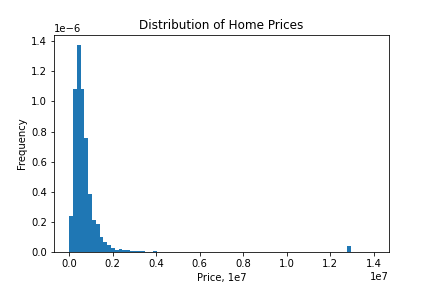
\includegraphics[width=130mm]{priceHist.png}
\end{center}
\caption{\textbf{.}}
\label{fig:priceHist}
\end{figure}
\\
First, $price$, the dependent variable in the model was looked into. The histogram for $price$ showed peaks in price to be clustered. The histogram also showed a few outliers in the data that should be removed before conducting further analysis.

\clearpage
\begin{figure}[h]
\begin{center}
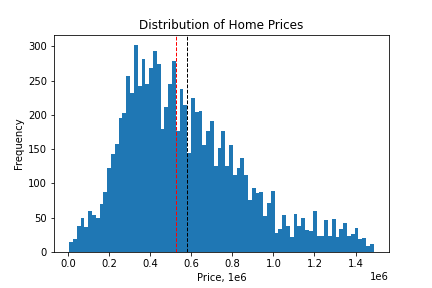
\includegraphics[width=130mm]{newPriceHist.png}
\end{center}
\caption{\textbf{.}}
\label{fig:NewpriceHist}
\end{figure}
After removing the necessary outliers, a new variable for price, newPrice, is created. Even though the histogram for newPrice shows that the average price for homes in the DC area is higher than the median price, the new price data is now more symmetrical than before. The peaks in the newPrice histogram show that most homes range between two-hundred and eight-hundred thousand dollars. \\
\clearpage

\tab This paper theorizes that the price premium decreases as the distance between a home in Washington D.C. and the nearest metro station increases. The histogram below shows the distribution of the homes by their proximity to the nearest metro station.

\begin{figure}[h]
\begin{center}
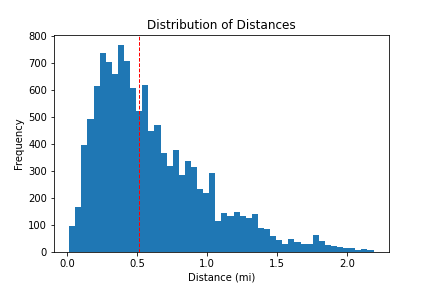
\includegraphics[width=130mm]{distanceHist.png}
\end{center}
\caption{\textbf{.}}
\label{fig:distanceHist}
\end{figure}
As observed in the Distance histogram, median homes are located within a 0.5-mile radius of the nearest metro station. The distribution is skewed to the right, with the distance ranging from zero to over two miles. Given that most homes are clustered within a one-mile radius, a dummy variable is created to see the difference in the price premium for homes within and outside the 0.5-mile radius to conduct further analysis.
\clearpage

\begin{figure}[h]
\begin{center}
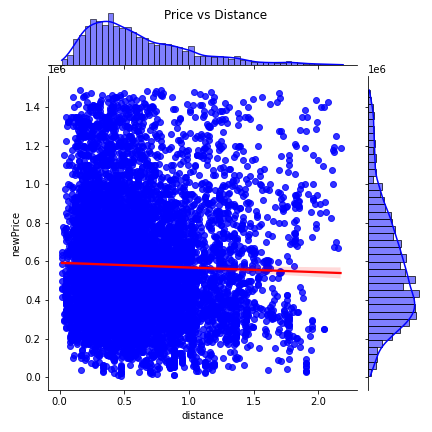
\includegraphics[width=110mm]{DistanceJoint.png}
\end{center}
\caption{\textbf{.}}
\label{fig:distanceJoint}
\end{figure}

The joint plot above shows the scatter plot of price and distance and the distribution of distance on the top, and the distribution of price on the right. The line of best fit in the scatterplot shows a clear downward sloping or negative relationship between the two variables. The downward sloping trend line shows that as the distance increases, the price of the homes decreases. 
\clearpage

To take a deeper look into the factors that affect home prices, it is important to take fixed effects and features of the homes into account.\\
\tab First, we looked at the number of bedrooms in the homes and its relationship with price.
\begin{figure}[h]
\begin{center}
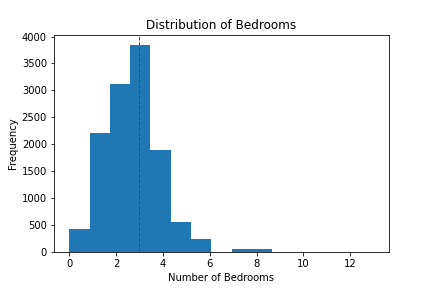
\includegraphics[width=130mm]{bedroomHist.png}
\end{center}
\caption{\textbf{.}}
\label{fig:bedHist}
\end{figure}
The histogram shows the median number of bedrooms in the dataset to be 3. The number of bedrooms ranges from one to six, with eight bedrooms being an outlier. 
\clearpage

\begin{figure}[h]
\begin{center}
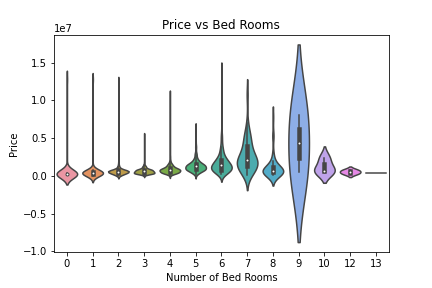
\includegraphics[width=130mm]{BedViolin.png}
\end{center}
\caption{\textbf{.}}
\label{fig:bedVio}
\end{figure}
When looking at this variable, it was expected that the price of the homes in D.C. would increase as the number of bedrooms increased. On the contrary, the white points in the violin plot show a steady increase in the median price as the number of bedrooms increases to five. At six bedrooms, the median price of homes begins to decline, and the price becomes constant at eight bedrooms. 
\clearpage


\begin{figure}[h]
\begin{center}
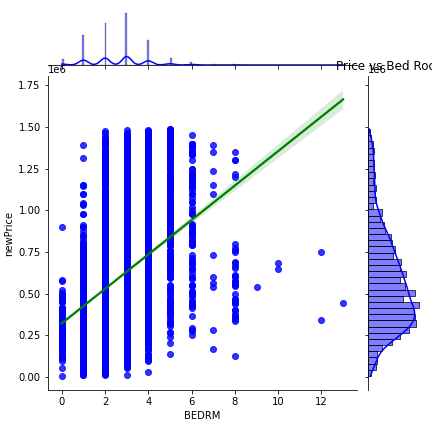
\includegraphics[width=130mm]{BedJoint.png}
\end{center}
\caption{\textbf{.}}
\label{fig:bedJoint}
\end{figure}
The joint plot for bedrooms and price shows the overall upward sloping line of best fit, which indicates a positive relationship between price and the number of bedrooms. It is also observed that the price peaks at around four-hundred thousand dollars in relation to the number of bedrooms. 
\clearpage

\begin{figure}[h]
\begin{center}
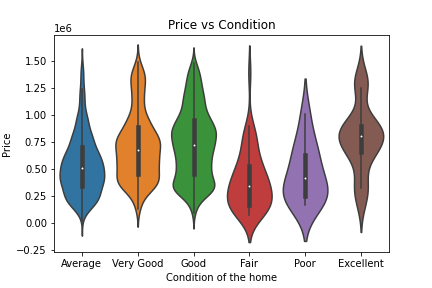
\includegraphics[width=130mm]{ConditionViolin.png}
\end{center}
\caption{\textbf{.}}
\label{fig:cndVio}
\end{figure}



\begin{figure}[h]
\begin{center}
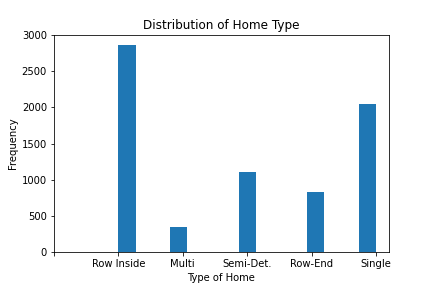
\includegraphics[width=130mm]{structureHist.png}
\end{center}
\caption{\textbf{.}}
\label{fig:strHist}
\end{figure}

\clearpage

\section*{Econometric Specification}
This paper utilizes a multiple linear regression approach using ordinary least squares estimators to predict if homes located within a half mile radius of a metro station incur a price premium. It is natural for homes to differ in price for several reasons, including size, year built, geographical location, or number of bedrooms. To determine if the metro station proximity is responsible for the differences in price, this paper controls for many home fixed effects mentioned above and in the data section.\\  \\
\tab This paper estimates four models, the first three utilize the price of a home as the demendent variable, denoted in dollars. The fourth equation estimates the price premium using the log of the home price to account for skew in the home price data. The general specification of the four models take on the functional form of Equation~\ref{eqn:1}.
\begin{align}
\ price = \beta_0 +\delta_1\ metro.5 + \beta_k\ (house\ fixed\ effects )+ u \ 
\label{eqn:1}
\end{align}
where $\delta_1$ is the paramater of interest and denotes the price differential for a house located within a half mild radius and a house located outside the radius. $metro.5$ is a dummy variable denoting whether a house falls within the radius: $metro.5$=1 if the house lies within the half mile radius and $metro.5$=0 if else.\\  \\
\tab The term house fixed effects encompasses the home attributes that do not change on average, including the number of bathrooms \& half-bathrooms, the lot size, the number rooms, the number of kitchens, and the type of structure.\\ \\
\tab In Model 4, this paper performs a stepwise selection process to determine which of the nine home fixed effects should be included in the final model. The stepwise selection independently estimates $price$ as a function of the nine home fixed effects and the $metro.5$ variable for a total of ten regressions. The term with the highest $R^2$ is added to the model, we call this $variable1$. Next, nine regressions are run, each with $variable1$ and the other eight variables; the term with the highest $R^2$ is added, we call this $variable2$. This process is repeated, adding the variable that results in the highest $R^2$ and removing variables that are not statistically significant. Model 4, estimates $\text{(log)}price$ as a function of the variables chosen by this method. \\ \\
\tab We expect the sign on $metro.5$ to be positive and moderately large as this paper hypothesizes that homes located within the half mile radius will be more expensive. We also expect the signs on $bedrooms$, $bathrooms$, $size$, $landarea$ to all be positive, indicating a higher price given more of these home attributes. We expect some of the structures to have a positive sign and others to have a negative sign, based on the style and quality of the structure. The results of the four regression models can be found in the next section.\\ \\
\tab To eliminate any multicollinearity issues, this paper examines a correlation matrix to identify independent variables that correlate with one another. Table~\ref{} illustrates the correlation matrix, with high values denoted in red.
\begin{table}[h!]
\centering
\begin{tabular}{|c| c | c |c |c |c |c |c | c | c|} 
\hline
\multicolumn{10}{|c|}{ \textbf{Correlation Matrix}} \\
\hline\hline
	&$\text{(log)}price$&	Price&	 struc. & metro50&	Stories&	Land&	Bath&	Rooms&	Half\\[0.5ex] \hline \  
$\text{(log)}price$&	1&	0.917&  -0.074& 	0.048& 0.170&	0.158& 0.480	& 0.357&	0.321\\ [0.5ex]\hline \ 
Price&	0.917& 	1&-0.040&	0.031& 	0.199& 	0.205& 	\textbf{\color{red}{0.524}}& 0.389&	0.348\\ [0.5ex]\hline\ 
sruc.& -0.074&	-0.040	& 1&	-0.146& 	-0.042	& \textbf{\color{red}{0.505}}&	0.136&	0.095&	0.099 \\ [0.5ex]\hline \  
metro50&	0.048	&  0.031&-0.146&	1&	0.014& 	-0.177&	-0.099&	-0.170&	-0.1050\\ [0.5ex] \hline \ 
Stories&	0.170	&  0.199&-0.042& 	0.014&	1&	-0.025&	0.033& 0.030&	0.031\\ [0.5ex]\hline \ 
Land&	0.158& 0.205&\textbf{\color{red}{0.505}}&	-0.177&	-0.025&	1&	0.420	& \textbf{\color{red}{0.505}}&	0.306\\ [0.5ex] \hline \ 
Bath&	0.480& 	\textbf{\color{red}{0.524}}&0.136& 	-0.099&	0.033& 	0.420&1&	\textbf{\color{red}{0.694}}& 	0.290\\ [0.5ex]\hline \ 
Rooms&	0.357& 	0.389&0.095 & 	-0.170&	0.030& \textbf{\color{red}{0.506}}&	\textbf{\color{red}{0.694}}&	1&	0.396 \\ [0.5ex]\hline \ 
Half&	0.321& 	0.348&0.099& 	-0.105&	0.031&	0.306&	0.290& 	0.3963&	1 \\ [0.5ex]\hline
\hline
\end{tabular}
\caption{\footnotesize Values above 0.50 are highlighted in red. Note that the correlation between log(price) and Price are not considered as they do not appear in the same model.}
\label{table:1}
\end{table}


$$price = \beta_0 +\delta_1\ nearMetro + \beta_1\ medianInc + \beta_2\ crimeRate + \beta_3\ bdrms + \beta_4\ stories + \beta_5\ sqft +$$$$ \beta_6\ fullBath + \beta_7\ halfBath + \beta_8\ grade + \beta_9\ landSize + u$$\\\\
where $nearMetro$ is a dummy variable; 1 if within a .5 mile radius from a metro station, $crimeRate$ is percentage of the crime per 100,000, $stories$ is the number of stories a house has, $sqft$ is the square feet of the home, among other home effects variables. \\


$$price = \beta_0 +\delta_1\ metro.5  + u$$
\bigskip
\bigskip

$metro.5=1$ if the house is within a 0.50 mile radius, 0 else



\bigskip
\bigskip
\bigskip
\bigskip

$$\text{log}(price) = \beta_0 +\delta_1\ metro.5  + \beta_1\ stories + \beta_2\ landArea + $$$$\beta_3\ cndtn + \beta_4\ bathroom + \beta_5\ AC + \beta_6\ bedroom + \beta_7\ halfbath + u $$

\bigskip
\bigskip
$metro.5=1$ if the house is within a 0.50 mile radius, 0 else




$$price = \beta_0 +\delta_1\ metro.5 + \beta_k\ (house\ fixed\ effects )+ u$$
\bigskip
\bigskip

parameter of interest: $\delta_1$\\
\tab \  $metro.5=1$ if the house is within a 0.50 mile radius, 0 else

\section*{Results}
\begin{table}[h!]
\centering
\begin{threeparttable}

\caption{Post Treatment Effects on $\text{NO}_\text{x}$}
\begin{tabular}{lccccc} 
%\multicolumn{6}{c}{ \textbf{DinD Treatment Effects on NOx}} \\
\hline\hline\\[0.001ex]
         &           \multicolumn{4}{c}{$Price$} &                        \multicolumn{1}{c}{Log($Price$)}                 \\ [0.1ex] \cline{2-4} \cline{6-6}  
\\[0.001ex]
         &                   (1) &              (2) &                      (3) &&                            (4) \\ [0.5ex] 
\hline \\[0.1ex]
Intercept&	574364.70\footnotesize***&	189648.32\footnotesize***&	248707.05&&	17.70\footnotesize*** \\
&	\footnotesize[-3424.27]&	\footnotesize(19850.63)&	\footnotesize(263607.00)&&	\footnotesize[0.10] \\
metro50&	24776.83\footnotesize***&	97631.25\footnotesize***&	96892.24\footnotesize***&&	0.21\footnotesize*** \\
&	\footnotesize[8176.48]&	\footnotesize(12838.28)&	\footnotesize(12821.84)&&	\footnotesize[0.03] \\
Stories&	&	63388.06\footnotesize***&	64507.54\footnotesize***&	 \\
&	&	\footnotesize(8460.41)&	\footnotesize(8447.44)	&& \\
Land&	 &	7.84\footnotesize***&	9.04&	& \\
&	&	\footnotesize(2.52)&	\footnotesize(2.53)&	& \\
Bedroom&	&	150960.90\footnotesize***&	143963.93\footnotesize***&&	0.32\footnotesize*** \\
&	&	\footnotesize(4490.45)&	\footnotesize(4717.21)&&	\footnotesize[0.01]\\
Half&	&	94667.83\footnotesize***&	87127.34\footnotesize***&&	0.24\footnotesize*** \\
&	&	\footnotesize(6886.83)&	\footnotesize(7053.45)&&	\footnotesize([0.02]\\
Multi&	&	-331169.10\footnotesize***&	-309597.28\footnotesize***&&	-0.78\footnotesize*** \\
&	&	\footnotesize(18996.8)2&	\footnotesize(19493.71)&&	\footnotesize[0.06] \\
Detached&	&	-190811.19\footnotesize***& -197509.55\footnotesize***&&	-0.54\footnotesize*** \\
&	&	\footnotesize(11459.7)8&	\footnotesize(11522.49)&&	\footnotesize[0.03] \\
Row&	 &	-52120.28\footnotesize***&	-57029.36\footnotesize***&& 	-0.17\footnotesize*** \\
&	&	\footnotesize(12490.2)4&	\footnotesize(12507.49)&&	\footnotesize[0.03] \\
Single&	&	-77761.28\footnotesize***&	-83945.82\footnotesize***&&	-0.25\footnotesize*** \\
&	&	\footnotesize(13528.3)0&	\footnotesize(13562.47)&&	\footnotesize[0.03]\\
Rooms&	&	&	&&	0.16\footnotesize***\\
&	&	&	&&	\footnotesize[0.02] \\
$Rooms^2$&	&	&	&&	-0.01\footnotesize*** \\
&	&	&	&&	\footnotesize[0.00] \\
$Bed^2$&	&	&	&&	0.005\footnotesize*** \\
&	&	&&	&	\footnotesize[0.00] \\
Fixed Effects &       Yes&             Yes &                  Yes &  &                       Yes    \\ [0.5ex]
Stepwise &       No&             No &                   No &  &                      Yes    \\ [0.5ex]
Observations&            9176 &           4825&                  4825   &&                         4834      \\ [0.5ex]
$R^2$ &                     0.001 &          0.381&                   0.327 &&                      0.321 \\ [0.5ex]
Adj-$R^2$&                 0.001&        &                  0.326 &  &                   0.320   \\ [0.5ex]
\hline
\bottomrule
\end{tabular}
\begin{tablenotes}
  
 \item \footnotesize{Notes. Each column reports results from a regression of dummy variables and other indicators for $Price$. Column (1),  Column (2), and Column (3) use the price of homes denoted in US dollars while Column (4) uses the log($Price$) as the demendent variable. Fixed effects include attributes to the homes that do not vary with time. Model 2 uses a general linear model while Model 1, 3, and 4 use ordinary least squares. The standard errors reported in square brackets  are robust standard errors. HC3 covariance methods are used in the ols model in python ($cov_type='HC3'$). $***p<.01. **<.05. *p<.10.$}

\end{tablenotes}
\label{table:5}
\end{threeparttable}
\end{table}
\clearpage


\section*{Analysis}
\section*{Further Research}
\section*{Conclusion}



\end{document}